%=========================================================================%
% - - KAPITOLA 4: Z Á S U V N Ý - M O D U L - I n R u n J U n i t V i e w %
\chapter{Implementovaná aplikace TestRunView}
\label{chapter:TRV}
%=========================================================================%
Díky architektuře zásuvných modulů je snadné rozšířit Eclipse IDE o~novou funkcionalitu a tak poskytuje četné množství prvků, které je vhodné otestovat. V~rámci testování GUI Eclipse IDE se používají rozsáhlé testovací sady testující velké množství aspektů a možností. Automatické testy GUI jsou ale časově náročné a nejsou dokonalé. Vzniká tak potřeba kontroly nad sadou s~probíhajícími testy. Průběh testů lze sledovat pomocí zásuvného modulu \texttt{org.eclipse.jdt.junit}, který poskytuje pohled JUnit zobrazující potřebné informace o~probíhajících testech. Navíc umožňuje znovu spustit testovací sadu a také si uchovává historii testovaných sad. Problémem tohoto pohledu je, že při spuštění testovací sady se otevírá nové okno s~testovanou instancí Eclipse IDE. To způsobí překrytí pohledu JUnit a proto není možné sledovat tento pohled v~průběhu testování. Také z~hlediska časové náročnosti může být výhodnější testovat na vzdálených serverech a spouštět testy z~terminálu. V~takovém případě nelze pohled JUnit k~zobrazení detailů o~testování použít.

Implementovaná aplikace \emph{TestRunView} (dále zkráceně TRV) poskytuje možnost zobrazení informací o~probíhajícím testování GUI Eclipse IDE bez narušení průběhu testů. Mezi důležité informace které tato aplikace zobrazuje patří zobrazení průběhu a výsledků jednotlivých testovacích případů v~rámci spuštěné testovací sady. V~případě nějaké chyby v~testovací sadě potom lze lépe prozkoumat kde chyba nastala a jaká byla její příčina.

Tato kapitola detailně popisuje architekturu, implementaci, způsob testování a využití této aplikace.

  \section{Návrh architektury aplikace TestRunView}
  %================================================

  V~rámci návrhu bylo třeba zvážit způsoby, jakými lze data o~probíhajících testech získávat a jakými lze tyto data zobrazovat. Ve společnosti \emph{Red Hat} se používají pro testování rámce JUnit a \emph{RedDeer}\footnote{\url{https://github.com/jboss-reddeer}}. RedDeer je rámec pro testování zásuvných modulů Eclipse IDE a využívá k~tomu rámec JUnit. Pomocí implementace vlastního \emph{runneru} dostává kontrolu nad probíhajícími testy. To umožňuje definovat například pořadí a typ spuštěných testů, nebo vytvářet vlastní anotace a tak definovat nové fáze probíhající v~rámci testování.

  Data tedy lze získávat z~obou zásuvných modulů\,--\,JUnitu i RedDeeru. JUnit ovšem narozdíl od RedDeeru poskytuje možnost připojit se pomocí bodu rozšíření\\\texttt{org.eclipse.jdt.junit.testRunListeners} a tak umožňuje širší použití výsledné aplikace. Vytvořený zásuvný modul není třeba explicitně přidávat v~kódu rámce nebo testů, ale je automaticky spuštěn.
  \\
  \\
  \noindent
  Možností jak zobrazit informace zachycené z~zásuvného modulu JUnit je několik:
  \begin{enumerate}
   \item pomocí pohledu\,(nebo jiné komponenty Eclipse Workbench) přímo v~instanci Eclipse IDE s~běžícími testy
   \item pomocí externí aplikace
   \item pomocí nástrojů operačního systému\,(notifikace, terminál)
  \end{enumerate}

  Při zobrazování dat je nutné aby nedocházelo k~narušování běhu testů a zároveň byly informace o~běžících testech viditelné. V~případě zobrazování informací o~probíhajících testech přímo v~testované instanci Eclipse IDE by bylo velmi problematické zajistit oba tyto případy. Zobrazení informaci pomocí nástrojů operačního systému by sice umožňovalo nenarušený běh testů, ale přehlednost zobrazených výsledků by byla pravděpodobně nižší. Proto je zobrazení výsledků implementováno pomocí externí SWT aplikace, která umožňuje nenarušený průběh testů a komfortní zobrazení výsledků.

  Velmi důležitou částí návrhu je způsob předávání dat mezi částí získávající informace o~testech a částí, která tyto informace zobrazuje. To lze řešit například externím souborem nebo pomocí síťové komunikace typu klient-server. V~aplikaci je z~důvodu možnosti připojení klientské aplikace k~vzdálenému serveru zvolen způsob komunikace typu klient-server.

  Aplikace TRV se skládá ze dvou samostatných částí\,--\,zásuvného modulu InRunJUnit a SWT aplikace TRView\,(viz obrázek \ref{fig:TRV_architecture}). InRunJUnit je nainstalován jako jeden ze zásuvných modulů platformy Eclipse a slouží k~získání a zpracování výsledků ze zásuvného modulu JUnit. Zároveň slouží jako server, ke kterému lze připojovat klientské aplikace. TRView zpracovává a zobrazuje data o~probíhajících testech uživateli. Tyto data získává pomocí soketů přijatých ze serveru. \emph{JDT}\,(\emph{Java Development Tools}) a \emph{PDE}\,(\emph{Plug-in Development Environment}) jsou zásuvné moduly, které rozšiřují funkcionalitu platformy Eclipse\,--\,JDT přidává nástroje pro práci s~Javou a PDE přidává funkcionalitu potřebnou pro vývoj zásuvných modulů. Platforma Eclipse je popsána v~kapitole \ref{chapter:eclipse_ide}.

  \begin{figure}
    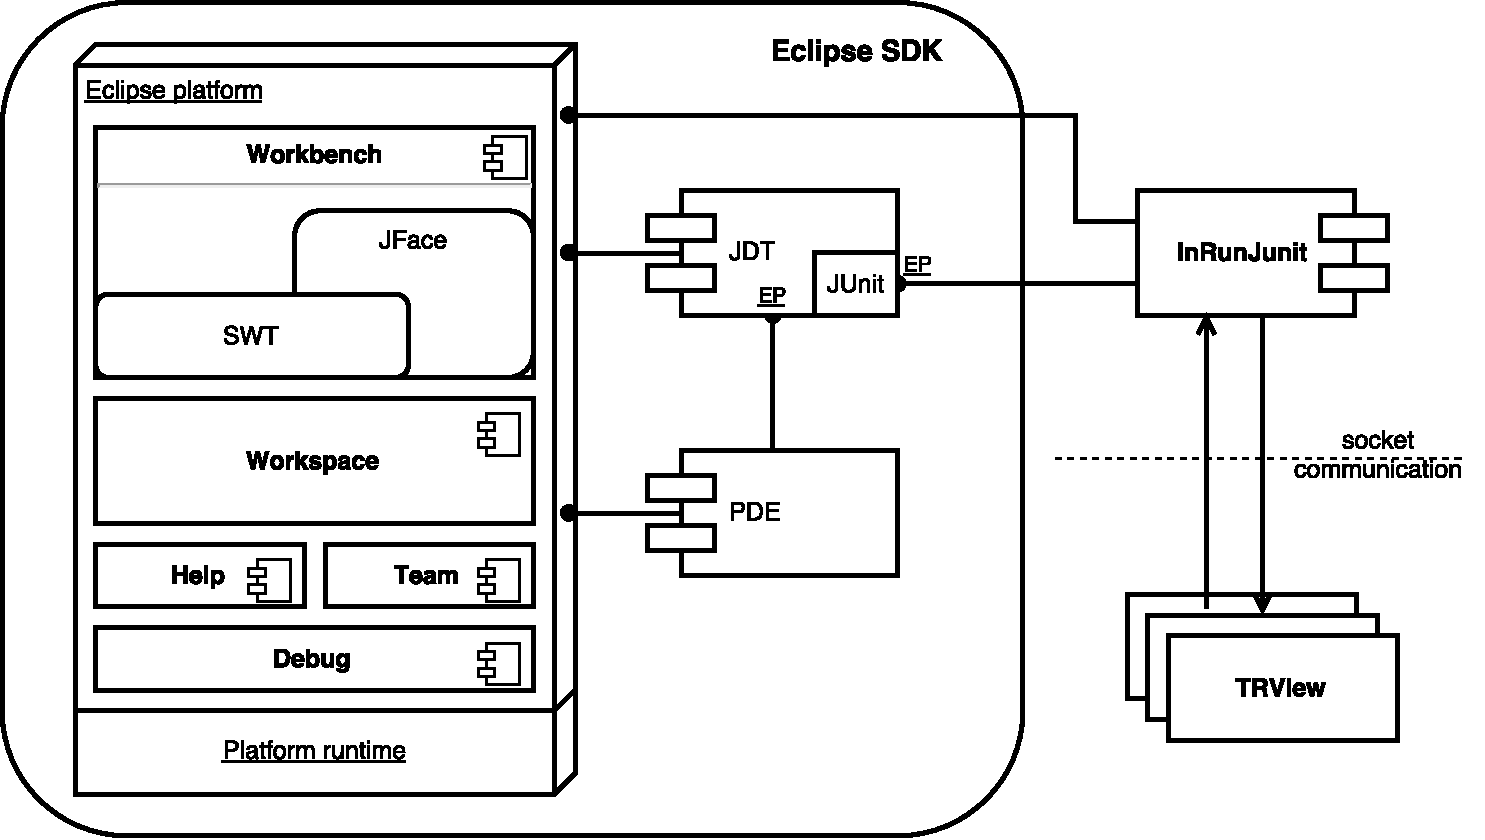
\includegraphics[width=\textwidth, center]{obrazky-figures/TRV_architecture.pdf}
    \caption{Znázornění architektury aplikace TRV.}
    \label{fig:TRV_architecture}
  \end{figure}

    \subsection{Návrh architektury zásuvného modulu InRunJUnit}
    Integrace zásuvného modulu InRunJUnit do platformy Eclipse je znázorněna na obrázku \ref{fig:inrunjunit_eclipse_integration}. Zásuvný modul se skládá ze dvou částí\,--\,\emph{listeneru} a serveru. Listener slouží pro zachycení výsledků ze zásuvného modulu JUnit. Opakem listeneru je potom \emph{notifier}, jehož účelem je informovat listener o~nových datech. Listener je pomocí bodu rozšíření poskytovaného zásuvným modulem JUnit zaregistrován mezi ostatní listenery. Poté, co se spustí JUnit za účelem testování, si JUnit zjistí které zásuvné moduly jsou k~bodu rozšíření připojeny a automaticky je informuje o~průběhu testů. Server se stará o~vytvoření serveru, komunikaci s~klienty, vytvoření relevantních dat ve formě řetězce a jejich posílání všem připojeným klientům. Při posílání dat také specifikuje fázi testování\footnote{Může se jednat o~zahájení (případně ukončení) testovací sady nebo testovacího případu.}, ze které data pochází.

      \begin{figure}
	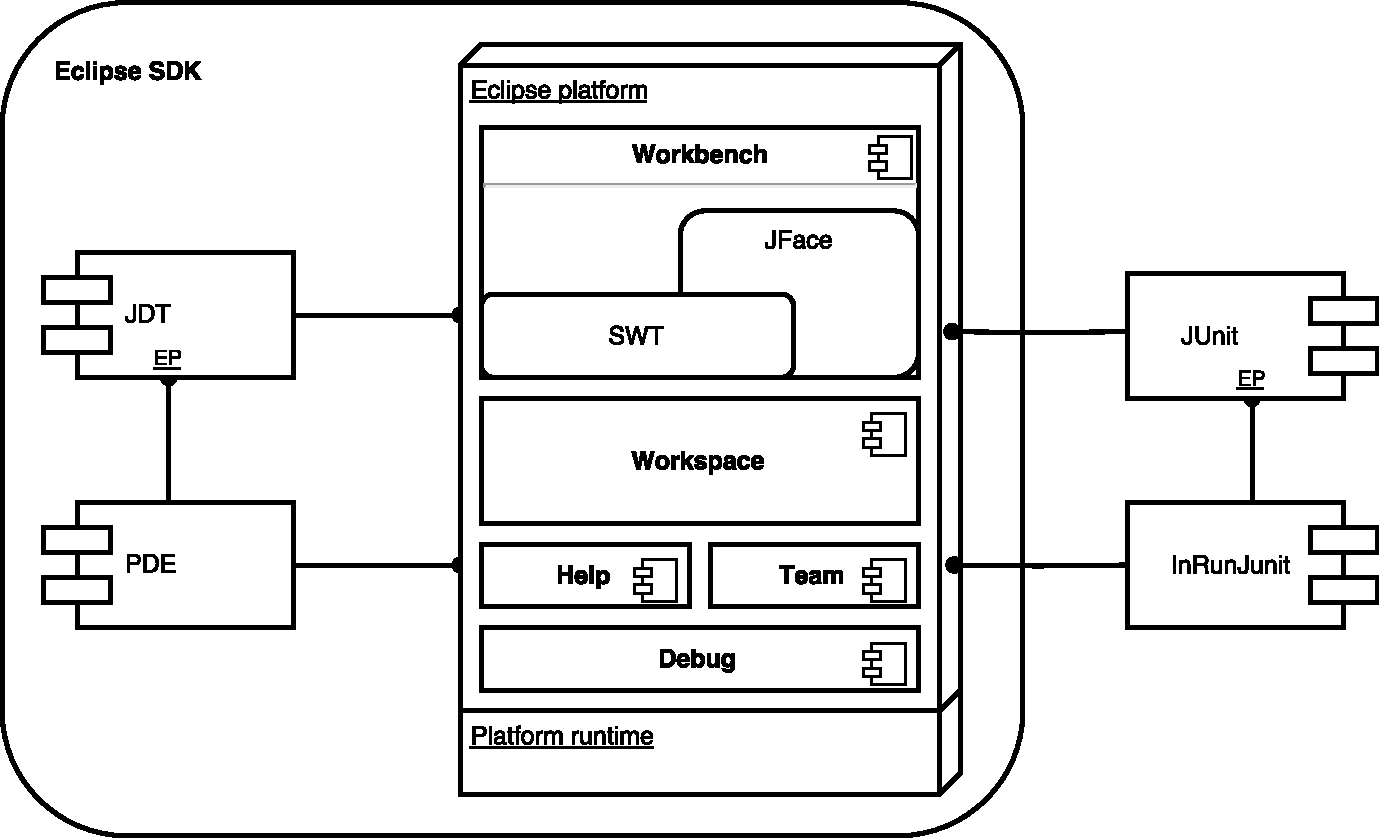
\includegraphics[width=\textwidth, center]{obrazky-figures/inrunjunit_eclipse_integration.pdf}
	\caption{Znázornění integrace zásuvného modulu InRunJUnit v~platformě Eclipse.}
	\label{fig:inrunjunit_eclipse_integration}
      \end{figure}

    \subsection{Návrh architektury aplikace TRView}
    Aplikace TRView se také skládá ze dvou částí\,--\,klienta a GUI. Klientská část umožňuje připojení k~serveru a ukládání přijatých výsledků. Při přijetí dat ze serveru také inicializuje zpracování a zobrazení průběhu testů do GUI. GUI se stará o~vytvoření a obsluhu grafického uživatelského rozhraní\,--\,obsahuje komponenty sloužící pro připojení k~serveru a zobrazuje důležité informace o~průběhu testů. To zahrnuje:
    \begin{itemize}
     \item pole pro zadání adresy a portu serveru
     \item počet testovacích případů, které poběží
     \item počet testových chyb (\emph{angl. failures}) v~testech
     \item počet běhových chyb (\emph{angl. errors}) v~testech
     \item počet přeskočených testů
     \item stromovou strukturu jednotlivých testovacích případů s:
     \begin{itemize}
      \item rozlišením který test je aktivní
      \item rozlišením výsledku testovacího případu
      \item časem udávajícím trvání testovacího případu
     \end{itemize}
     \item zobrazení \emph{stack strace} pro neúspěšné testy
    \end{itemize}

    \noindent
    V~případě, že testy a klientská aplikace poběží na jednom systému, je třeba vzít v~úvahu problém aktivního okna. Některé testy vyžadují pro nalezení a otestování komponent aktivitu daného okna. To může způsobit překrytí okna aplikace TRView a tak znemožnit zobrazení informací o~probíhajících testech uživateli. Proto je okno aplikace TRView vytvořeno \uv{vždy nahoře}(\emph{angl. always on top}). Okno je tak vždy viditelné, i když není právě aktivní.

    \subsection{Integrace zásuvného modulu InRunJUnit a SWT aplikace TRView}
    Komunikace mezi zásuvným modulem InRunJUnit a aplikací TRView je velmi důležitou částí návrhu. Ovlivňuje spoustu klíčových aspektů výsledné aplikace, které je třeba zvážit:
    \begin{itemize}
     \item rychlost komunikace
     \item možnost komunikace po síti
     \item počet možných klientů\,(instancí aplikace TRView) připojených k~zásuvnému modulu InRUnJUnit
     \item oboustrannost komunikace
    \end{itemize}
    
    \noindent
    V~aplikaci TRV je komunikace vyřešena pomocí klient-server modelu předávajícího informace pomocí soketů. Tento přístup poskytuje jednoduché a zároveň kompletní řešení uvedených problémů. Zpracováním dat v~zásuvném modulu InRunJUnit lze posílat pouze relevantní data a tak minimalizovat objem posílaných dat a zrychlit komunikaci. Navíc tento model umožňuje připojení klientské aplikace po síti a řeší tak jednoduše problém s~aktivitou oken. Díky paralelnímu programování lze připojit více klientských aplikací a zároveň umožnit oboustrannou komunikaci mezi všemi klienty a serverem. Oboustranná komunikace slouží k~korektnímu ukončování jak serveru, tak klienta. V~případě ukončení klienta je nutno oznámit serveru, že tomuto klientovi již nemá posílat data. V~případě ukončení serveru je nutno oznámit všem klientům, že nemají čekat na další data. Oboustrannou komunikaci by však bylo možno využít i pro budoucí rozšíření, například pro kontrolu běhu testů z~klientské aplikace.
    
    \begin{figure}
      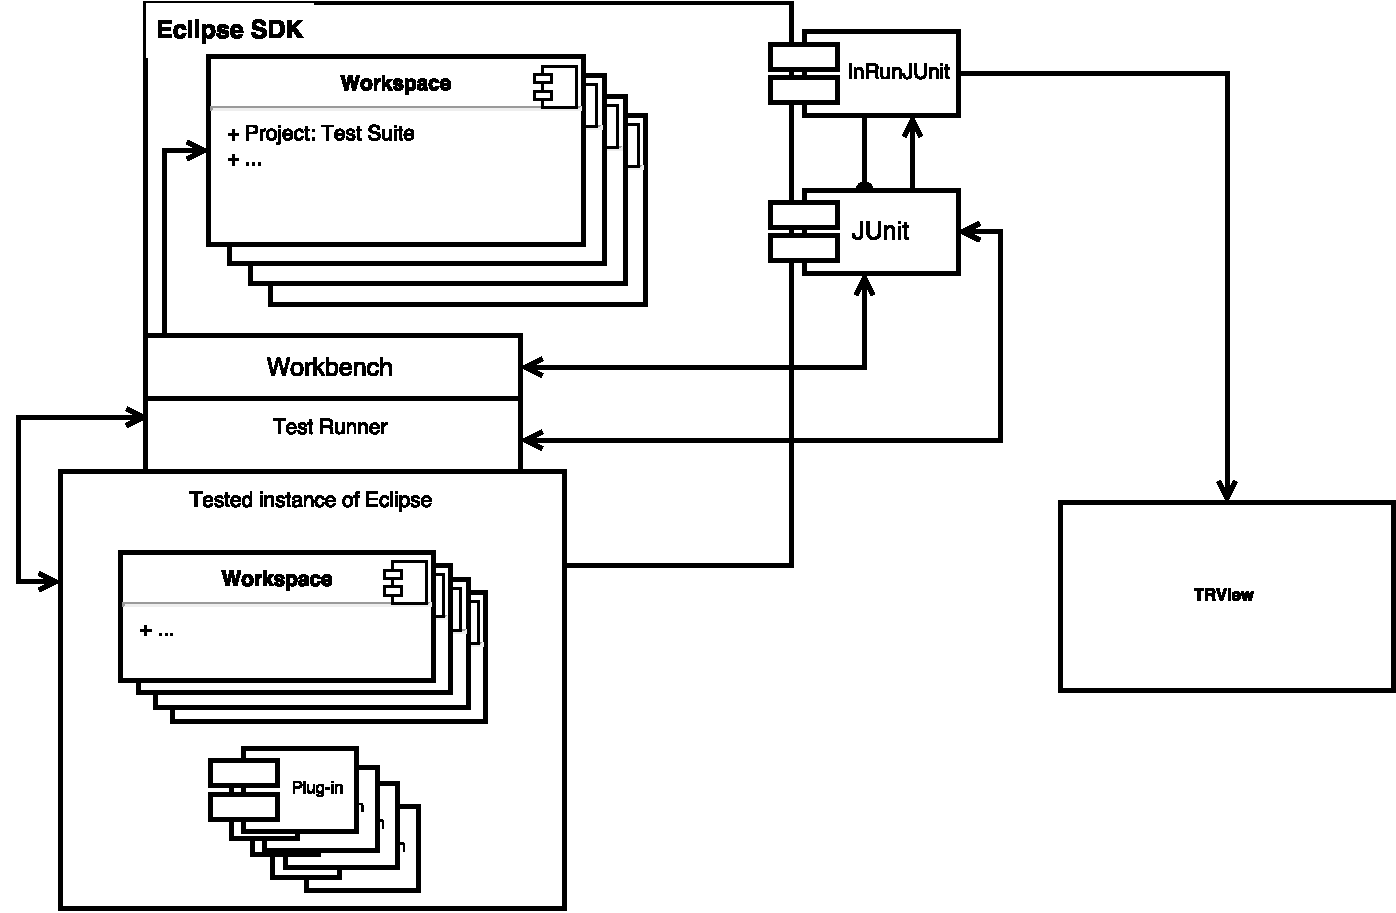
\includegraphics[width=\textwidth, center]{obrazky-figures/TRV_run_from_gui.pdf}
      \caption{Znázornění funkce aplikace TRV při spuštění testů z~GUI Eclipse IDE.}
      \label{fig:TRV_run_from_gui}
    \end{figure}


  \section{Implementace aplikace TRV}
  %==================================
  Aplikace TRV je implementována v~programovacím jazyce Java. Programovací jazyk Java byl vybrán na základě nutnosti implementace zásuvného modulu pro Eclipse IDE a následné komunikace s~externí aplikací. Vývoj aplikace probíhá pomocí verze \emph{JavaSE-1.8} a je doporučeno tuto verzi pro další vývoj nebo testování používat.

    \subsection{Implementace zásuvného modulu InRunJUnit}
    Součástí implementace zásuvného modulu je vytvoření manifestů zásuvného modulu, implementace listeneru a implementace serverové části. Více o~funkci manifestů a architektuře zásuvných modulů je uvedeno v~kapitole \ref{chapter:eclipse_ide}.
      
      \subsubsection{Manifesty zásuvného modulu InRunJUnit}
	Manifesty zásuvného modulu slouží jako zdroj základních informací pro platformu Eclipse. V~souboru \texttt{MANIFEST.MF} jsou data poskytující základní informace o~daném modulu (viz obrázek \ref{code:manifest.mf}). Informace \texttt{Manifest-Version}, \texttt{Bundle-ManifestVersion}, \texttt{Bundle-Name}, \texttt{Bundle-SymbolicName}, \texttt{Bundle-Version} slouží pro popis manifestu a jednoznačnou identifikaci zásuvného modulu a z~hlediska implementace nejsou příliš zajímavé. \texttt{Require-Bundle} obsahuje seznam všech ostatních balíčků, které jsou vyžadovány pro správné fungování zásuvného modulu. Za každým balíčkem může být ještě specifikována konkrétní verze balíčku, který je vyžadován. Balíčky uvedené na obrázku \ref{code:manifest.mf} slouží poskytují některé metody a třídy, které byly použity k~implementaci listeneru a serveru. Poslední uvedený balíček\,--\,\texttt{org.jboss.reddeer.common}\,--\,je zde kvůli logování aplikace za účelem testování aplikace. \texttt{Bundle-RequiredExecutionEnvironment} specifikuje prostředí pro provádění aplikace\,--\,JavaSE verze 1.8. 
	
	\lstset{language=}
	\begin{figure}
	  \begin{lstlisting}[frame=single]
Manifest-Version: 1.0
Bundle-ManifestVersion: 2
Bundle-Name: InRunJUnit
Bundle-SymbolicName: com.mcoufal.inrunjunit;singleton:=true
Bundle-Version: 1.0.0.qualifier
Require-Bundle: org.junit;bundle-version="4.12.0",
  org.eclipse.core.runtime;bundle-version="3.12.0",
  org.eclipse.debug.ui;bundle-version="3.11.201",
  org.eclipse.jdt.core;bundle-version="3.12.1",
  org.eclipse.jdt.junit.core,
  org.jboss.reddeer.common
Bundle-RequiredExecutionEnvironment: JavaSE-1.8
	  \end{lstlisting}
	  \caption{Zdrojový kód manifestu MANIFEST.MF obsahující základní informace o~zásuvném modulu InRunJUnit.}
	  \label{code:manifest.mf}
	\end{figure}
	
	Manifest \texttt{plugin.xml} obsahuje pouze informaci, že třída \texttt{com.\-mcoufal.\-inrunjunit.\-listener.\-JUnitListenerEP} implementuje potřebné rozhraní pro bod rozšíření \texttt{org.\-eclipse.\-jdt.\-junit.\-testRunListeners} (viz obrázek \ref{code:plugin.xml}). Tato informace umožňuje, aby byl implementovaný listener načten a informován zásuvným modulem JUnit o~průběhu testování. První dva řádky specifikují pouze verzi jazyka XML, ve kterém je manifest zapsán a verzi Eclipse IDE, ve které byl zásuvný modul vyvíjen.  

	\lstset{language=xml}
	\begin{figure}
	  \begin{lstlisting}[frame=single]
<?xml version="1.0" encoding="UTF-8"?>
<?eclipse version="3.4"?>

<plugin>
  <extension point="org.eclipse.jdt.junit.testRunListeners">
    <testRunListener class=
    "com.mcoufal.inrunjunit.listener.JUnitListenerEP"/>
  </extension>
</plugin>
	  \end{lstlisting}
	  \caption{Zdrojový kód manifestu plugin.xml zásuvného modulu InRunJunit.}
	  \label{code:plugin.xml}
	\end{figure}
     
      \subsubsection{Implementace listeneru}
	Balíček \texttt{listener} obsahuje pouze jednu třídu Java\,--\,\texttt{org.\-mcoufal.\-inrunjunit.\-listener.\-JUnitListenerEP}. Funkce této třídy je znázorněna na obrázku \ref{fig:listener_flowchart}. Instance třídy JUnitListenerEP je automaticky vytvořena zásuvným modulem JUnit, a to díky deklaraci připojení k~bodu rozšíření \texttt{org.\-eclipse.\-jdt.\-junit.\-testRunListeners}. Při inicializaci si tato instance vytváří nový server, který je obsluhován dalším vláknem. Metody listeneru jsou poté volány pokaždé, když začne příslušná fáze v~testování. To umožní při zavolání této metody zpracovat výsledky přijaté jako parametr dané metody a inicializovat jejich poslání pomocí dříve vytvořeného serveru. Pokud je zavolána metoda spojená s~koncem testovací sady, je po předání výsledků serveru zároveň inicializováno jeho ukončení.
	
	Nejdůležitějším krokem implementace třídy \texttt{JUnitListenerEP} je rozšíření třídy \texttt{org.\-eclipse.\-jdt.\-junit.\-TestRunListener}. Přepsáním (\emph{angl. override}) metod této třídy je dosaženo kontroly nad jednotlivými metodami, které rámec JUnit volá a tak informuje listener o~průběhu testování.
	
	\begin{figure}
	  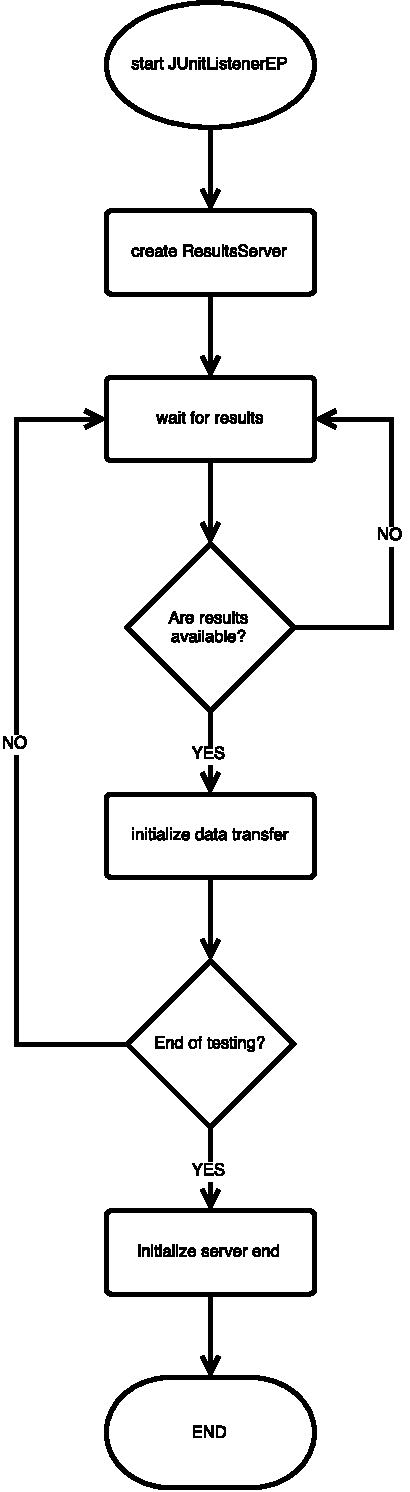
\includegraphics[width=\textwidth, height=0.8\textheight, keepaspectratio, center]{obrazky-figures/inrunjunit_listener_flowchart.pdf}
	  \caption{Diagram znázorňující funkci implementovaného listeneru \texttt{JUnitListenerEP} rozšiřujícího třídu \texttt{org.eclipse.jdt.junit.testRunListeners}.}
	  \label{fig:listener_flowchart}
	\end{figure}
      
      \subsubsection{Implementace serverové části}
	Hlavní třídou definující chování serveru je třída \texttt{ResultsServer} (viz obrázek \ref{fig:resultsserver_flowchart}). Tato třída má na starosti vytvoření serveru a správu klientů. Po vytvoření serveru na portu číslo 7357 se čeká na připojení klienta. Na každého připojeného klienta si ukládá odkaz a zároveň vytváří nové vlákno, které má na starosti obsluhu daného klienta. Tato obsluha je implementována ve třídě \texttt{ClientHandler}. Díky vytvořenému seznamu odkazů na jednotlivé klienty umožňuje třída \texttt{JUnitListenerEP} inicializovat posílání dat jednotlivým klientům a zároveň pomocí více vláken umožňuje obsluhu více klientů najednou. V~případě zachycení dat spojených s~ukončením testovací sady je po poslání dat server ukončen. Pro názornost je v~diagramu na obrázku ukončení serveru zaznačeno, ve skutečnosti však ukončení serveru probíhá asynchronně.
	
	\begin{figure}
	  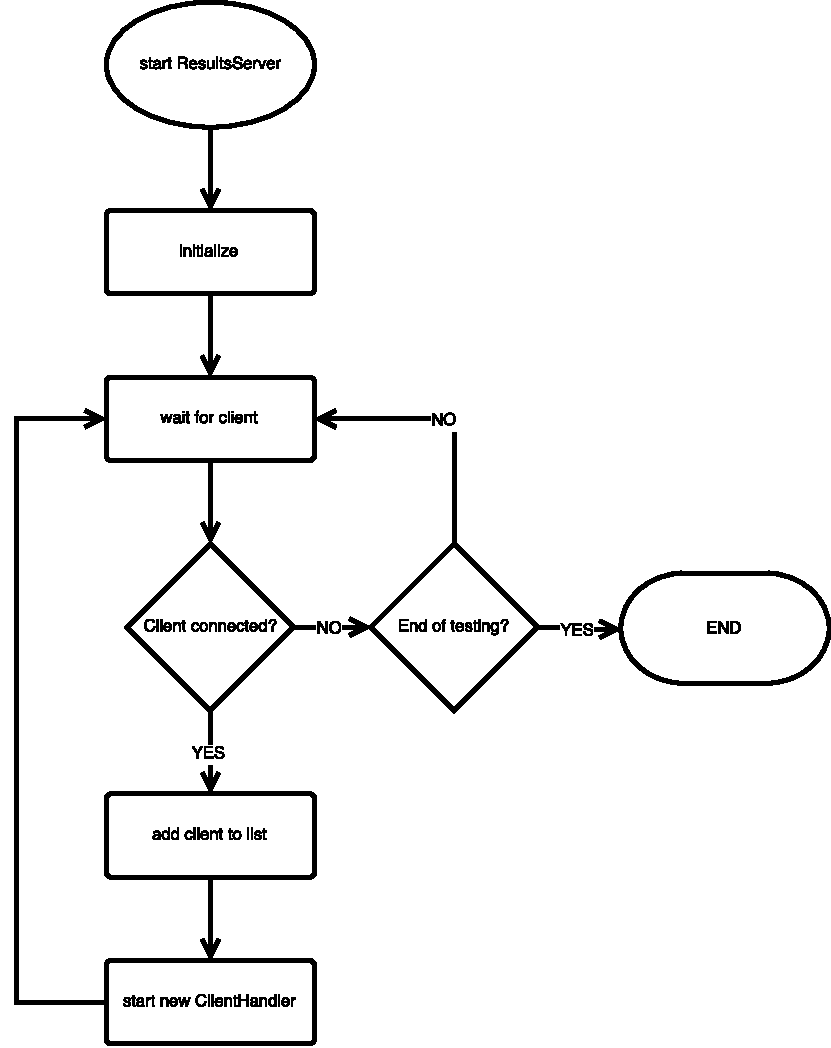
\includegraphics[width=\textwidth, height=\textheight, keepaspectratio, center]{obrazky-figures/inrunjunit_resultsserver_flowchart.pdf}
	  \caption{Diagram znázorňující funkci implementovaného serveru \texttt{ResultsServer} zajišťujícího komunikaci mezi zásuvným modulem InRunJUnit a aplikací TRView.}
	  \label{fig:resultsserver_flowchart}
	\end{figure}

	Hlavním účelem třídy \texttt{ClientHandler} je obsluha klienta a přenos dat (viz Obrázek \ref{fig:clientHandler_flowchart}). Jakmile dojde k~inicializaci a úspěšnému spojení s~klientem, posílá se počáteční soubor dat. Tento soubor obsahuje všechna data zachycená pomocí listeneru do doby, než došlo k~připojení klienta. Nedochází tak k~ztrátě dat v~případě, že se klient připojí až v~průběhu testů. Dále se již posílají jen nově zachycená data (odesílání těchto dat inicializuje \texttt{JUnitListenerEP} prostřednictvím instance \texttt{ResultsServer}). Díky tomuto modelu komunikace nedochází k~posílání irelevantních dat a zbytečnému zatížení síťové komunikace. Při zachycení dat z fáze ukončení testovací sady dojde k poslání dat klientovi a poté se ClientHandler ukončí.V případě ukončení uživatelem z grafického uživatelského rozhraní se nejdříve dojde k výjimce při posílání dat a ClientHandler se ukončí.

	\begin{figure}
	  \centering
	  \begin{minipage}{0.45\textwidth}
	    \centering
	    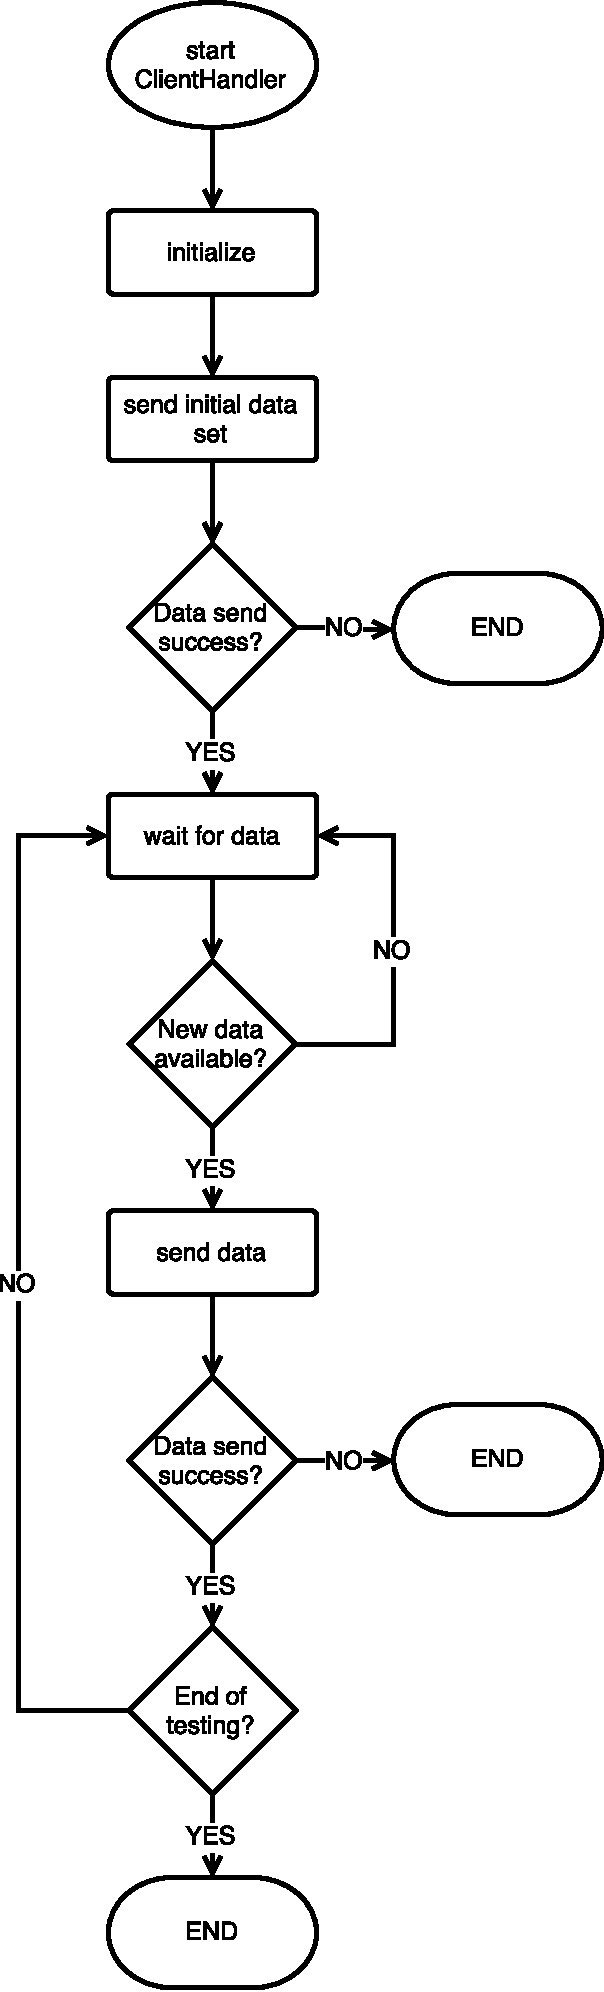
\includegraphics[width=0.9\textwidth, height=0.95\textheight, keepaspectratio, center]{obrazky-figures/inrunjunit_clienthandler_flowchart.pdf}
	  \caption{Diagram znázorňující funkci obsluhy klienta implementovanou v~třídě \texttt{ClientHandler}.}
	  \label{fig:clientHandler_flowchart}
	  \end{minipage}\hfill
	  \begin{minipage}{0.45\textwidth}
	    \centering
	    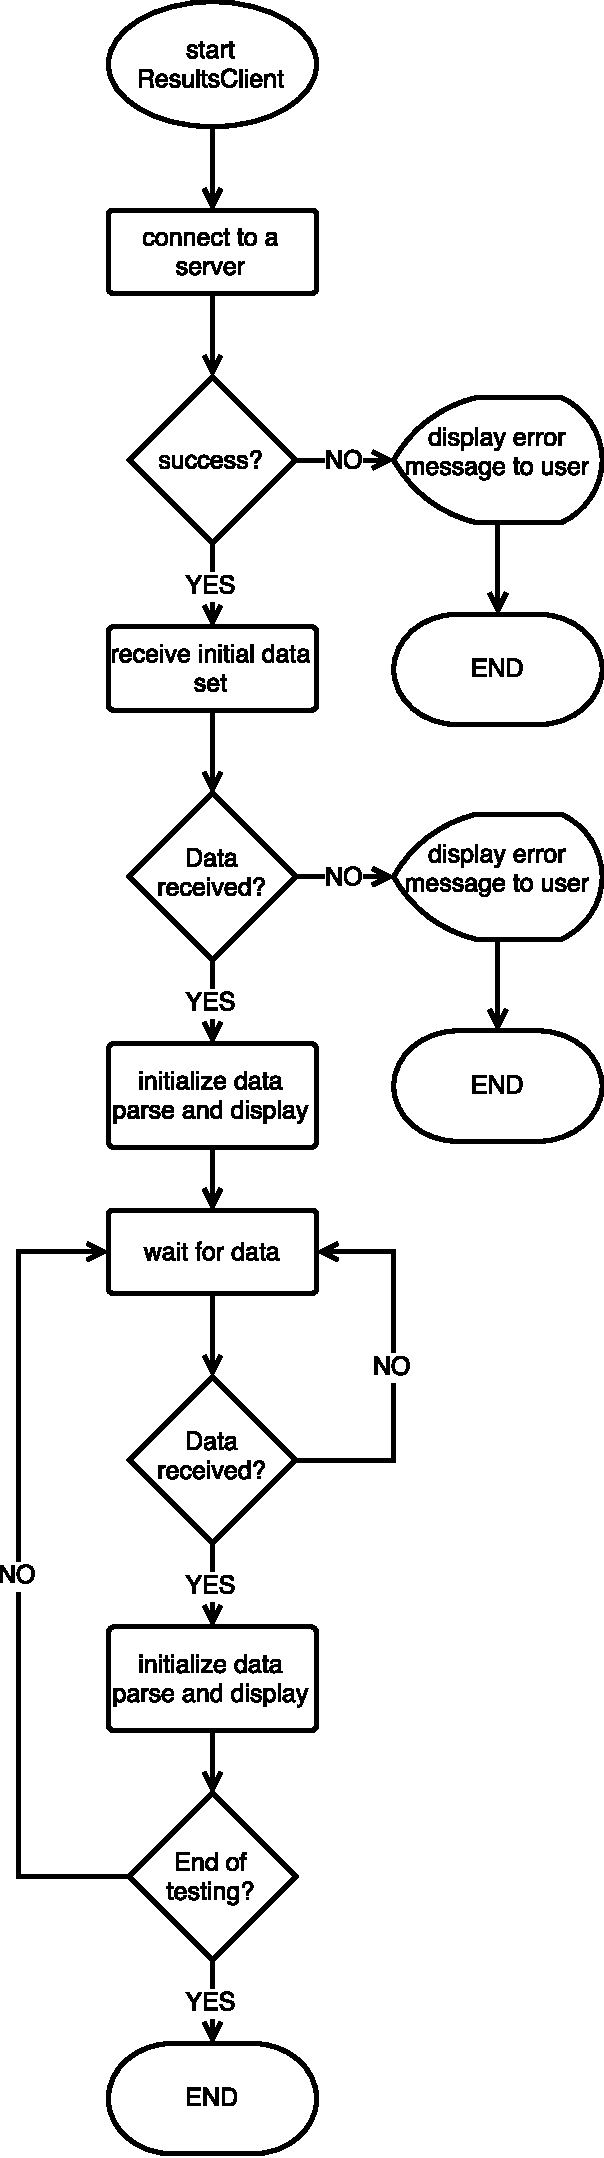
\includegraphics[width=0.9\textwidth, height=0.95\textheight, keepaspectratio, center]{obrazky-figures/trview_resultsclient_flowchart.pdf}
	  \caption{Diagram znázorňující chování implementovaného klienta \texttt{ResultsClient.}}
	  \label{fig:resultsclient_flowchart}
	  \end{minipage}
	\end{figure}
	
	Dále serverová část obsahuje pouze třídy použité pro zpracování a posílání dat. Cílem těchto tříd je uložení potřebných informací do serializovatelné formy. Dosáhneme tak zmenšení objemu posílaných a jednoduššího zpracování dat v~klientské aplikaci. Hlavní třídou pro manipulaci s~výsledky je třída \texttt{ResultsData}. Ta obsahuje vždy instanci jednoho objektu a fázi, ve které byla data objektu zachycena. Díky fázi potom klient pozná, jak s~objektem nakládat při zpracování a zobrazení dat. Ostatní třídy se starají pouze o~uložení dat jednotlivých objektů do řetězcové nebo číselné podoby. Jedná se o~třídy \texttt{StringDescription}, \texttt{StringResult}, \texttt{StringTestCaseElement}, \texttt{StringTestElement}, \texttt{StringTestRunSession}.

    \subsection{Implementace aplikace TRView}
    Implementace aplikace TRView je rozdělena do dvou balíčků\,--\,\texttt{view} a \texttt{client}. Balíček \texttt{view} zajišťuje vytvoření a obsluhu grafického uživatelského rozhraní a zároveň poskytuje metody pro zpracování a zobrazení dat získaných pomocí balíčku \texttt{client}. Balíček \texttt{client} se stará o~komunikaci se serverem a inicializaci zobrazení dat uživateli. 
    
      \subsubsection{Implementace balíčku \texttt{view}}
      Balíček \texttt{view} obsahuje dvě třídy\,--\,\texttt{TRView} a \texttt{ResultsParser}. Třída \texttt{TRView} tvoří základ aplikace\,--\,inicializuje a vytváří grafické uživatelské rozhraní aplikace a definuje chování pro akce, které nastaly v~GUI (akce provedené uživatelem pomocí myši nebo klávesnice). Pokud uživatel zadá IP adresu a port serveru, na kterém běží testy, stiskem tlačítka \texttt{CONNECT} se resetuje GUI, ukončí se instance stávajícího klienta \texttt{ResultsClient} (pokud byl již nějaký vytvořen) a vytvoří se nové vlákno zajišťující jeho funkci. V~případě označení některého z~testovacích případů se zobrazí jeho stack trace. Pokud uživatel ukončí aplikaci, inicializuje se konec klienta \texttt{ResultsClient} a aplikace se ukončí. Chování implementované v~třídě TRView je znázorněno na obrázku \ref{fig:trview_flowchart}.

      \begin{figure}
	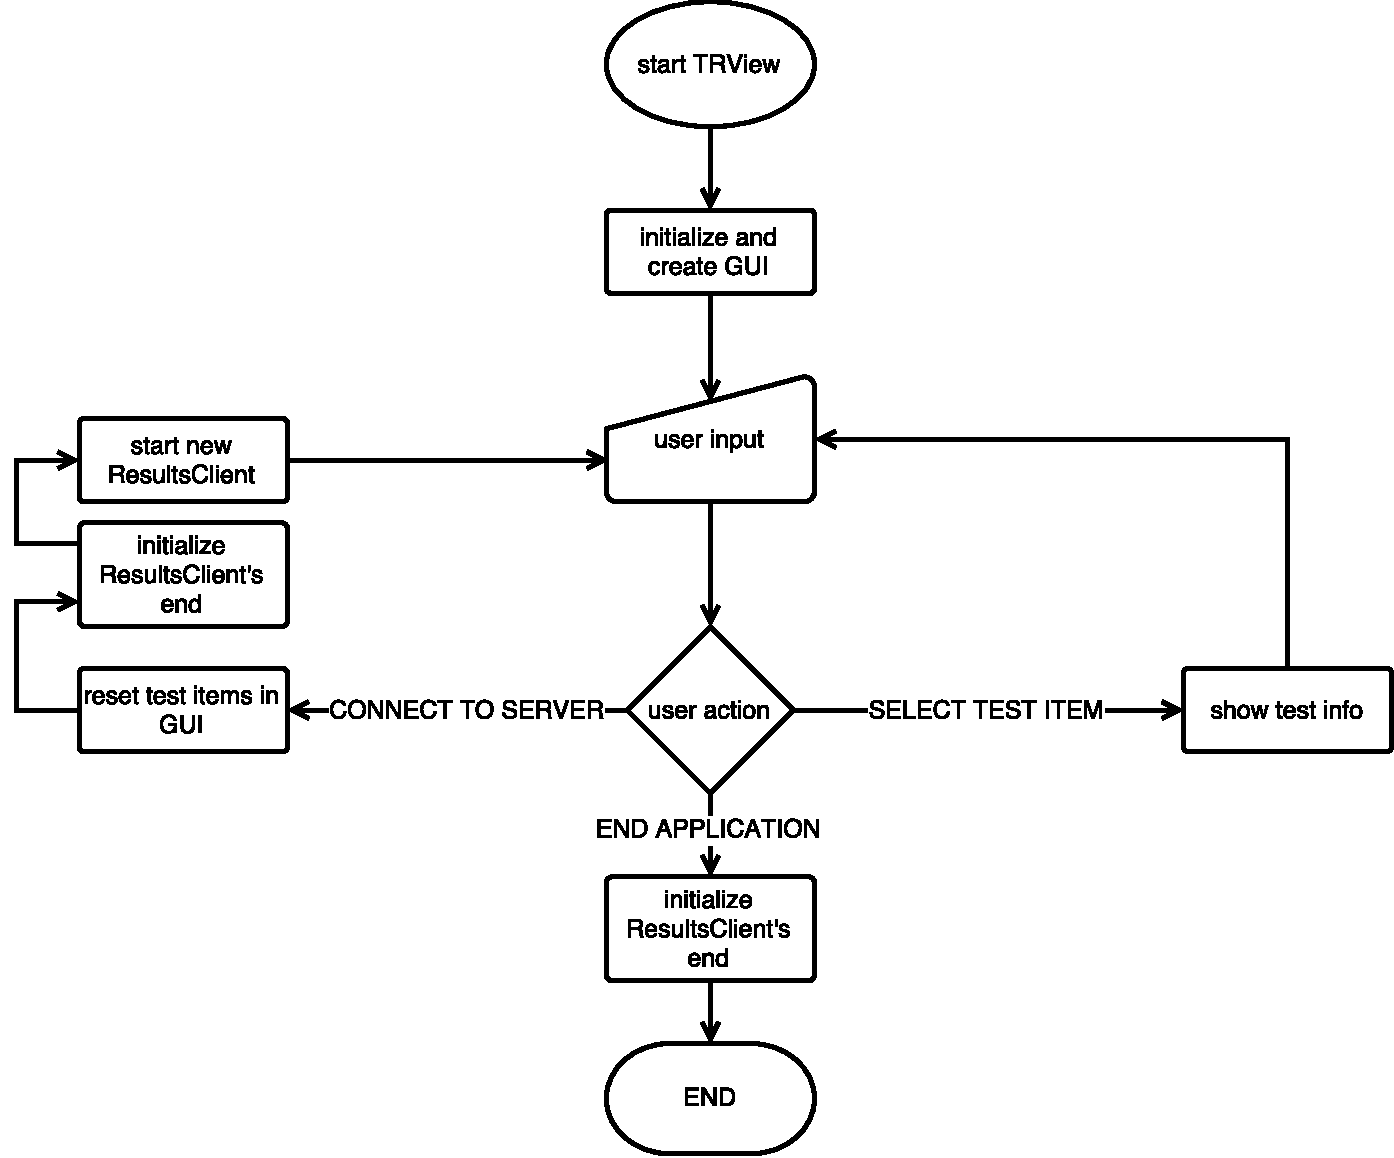
\includegraphics[width=\textwidth, height=\textheight, keepaspectratio, center]{obrazky-figures/trview_trview_flowchart.pdf}
	\caption{Diagram znázorňující funkci třídy TRView.}
	\label{fig:trview_flowchart}
      \end{figure}

      \begin{figure}
	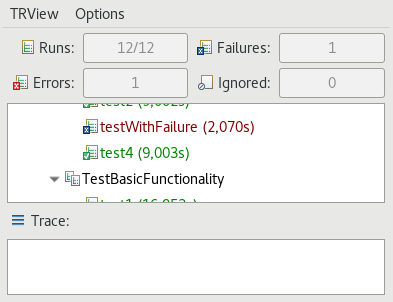
\includegraphics[width=\textwidth, center]{obrazky-figures/TRV_gui.png}
	\caption{Grafické uživatelské rozhraní implementované aplikace TRView.}
	\label{fig:TRV_gui}
      \end{figure}

      \noindent Grafické uživatelské rozhraní se skládá z:
      \begin{description}
	 \item[Menu:] obsahuje jednoduchou nabídku pro snadné ovládání aplikace. Nabídka obsahuje možnosti \texttt{Connect...}, \texttt{Re-connect}, \texttt{Disconnect} a \texttt{Exit}, sloužící pro připojení a opětovné přípojení k serveru, odpojení od serveru a ukončení aplikace.
	 \item[Popisků:] slouží k~identifikaci jednotlivých komponent (říkají tak uživateli, jaký je význam dat dané komponenty)
	 \item[Textových polí:] slouží pro zobrazení informací (počet chyb, běhů testů, atd.) nebo pro zadávání informací uživatelem (IP adresa serveru, port serveru).
	 \item[Stromová struktura:] je nejdůležitější část GUI aplikace. Do této struktury se zobrazuje průběh testů jednotlivých testovacích případů. Pro každý uzel ve stromu je zobrazena příslušná ikona (viz tabulka \ref{tab:trview_icons}) informující o~jeho stavu.
	 \item[Stack trace:] textový záznam zobrazující výpis metod které byly volány, než došlo u~vybraného testovacího případu k~chybě. Pokud žádná chyba nenastala, textové pole obsahuje pouze řetězec informující uživatele o~tom, že stack trace je prázdný.
      \end{description}

      \begin{table}
      \renewcommand{\tabularxcolumn}[1]{>{\small}m{#1}}
      \centering
      \begin{tabularx}{\textwidth}{|p{1cm}|X|}
	\hline
	\textbf{Ikona} & \textbf{Význam}\\ \hline
	\raisebox{-0.3\height}{
\includegraphics[width=1.5em, center]{ikony-icons/tsuite.png}} & Uzel obsahující testovací případy. Může se jednat o testovací sadu, balíček nebo testovací třídu.\\ \hline
	\raisebox{-0.3\height}{
\includegraphics[width=1.5em, center]{ikony-icons/tsuiterun.png}} & Testovací sada právě běží.\\ \hline
	\raisebox{-0.3\height}{
\includegraphics[width=1.5em, center]{ikony-icons/tsuiteok.png}} & Testovací sada proběhla v pořádku.\\ \hline
	\raisebox{-0.3\height}{
\includegraphics[width=1.5em, center]{ikony-icons/tsuiteerror.png}} & Testovací sada proběhla, nastalo v ní jedna nebo více běhových chyb.\\ \hline
	\raisebox{-0.3\height}{
\includegraphics[width=1.5em, center]{ikony-icons/tsuitefail.png}} & Testovací sada proběhla, nastalo v ní jedna nebo více testových chyb.\\ \hline
	\raisebox{-0.3\height}{
\includegraphics[width=1.5em, center]{ikony-icons/test.png}} & Uzel představující jeden testovací případ.\\ \hline
	\raisebox{-0.3\height}{
\includegraphics[width=1.5em, center]{ikony-icons/testrun.png}} & Testovací případ právě běží.\\ \hline
	\raisebox{-0.3\height}{
\includegraphics[width=1.5em, center]{ikony-icons/testok.png}} & Testovací případ proběhl v pořádku.\\ \hline
	\raisebox{-0.3\height}{
\includegraphics[width=1.5em, center]{ikony-icons/testerr.png}} & Testovací případ skončil s běhovou chybou.\\ \hline
	\raisebox{-0.3\height}{
\includegraphics[width=1.5em, center]{ikony-icons/testfail.png}} & Testovací případ skončil s testovou chybou.\\ \hline
	\raisebox{-0.3\height}{
\includegraphics[width=1.5em, center]{ikony-icons/testignored.png}} & Testovací případ neproběhl\,--\,byl přeskočen.\\ \hline
	\raisebox{-0.3\height}{
\includegraphics[width=1.5em, center]{ikony-icons/testassumptionfailed.png}} & Testovací případ skončil , stav je neznámý a předpokládá se chyba\\ \hline
      \end{tabularx}
      \label{tab:trview_icons}
      \caption{Seznam ikon použitých v grafickém uživatelském rozhraní aplikace TRView.}
      \end{table}

      Třída \texttt{ResultsParser} obsahuje metody, které na vstupu zpracovávají instance třídy \texttt{ResultsData} a zobrazují je do GUI. Díky fázi uvedené v~objektu \texttt{ResultsData} lze poznat, v~jaké fázi testování byla data zachycena a podle toho data zpracovat a zobrazit. Jednotlivé fáze jsou definovány v~třídě \texttt{JUnitListenerEP} zásuvného modulu InRunJunit.

      \subsubsection{Implementace balíčku \texttt{client}}
      Balíček \texttt{client} obsahuje pouze třídu \texttt{ResultsClient}. Funkce implementovaná touto třídou je znázorněna na obrázku \ref{fig:resultsclient_flowchart}. Instance třídy \texttt{ResultsClient} vzniká po zadání detailů připojení a stisku tlačítka \texttt{CONNECT} uživatelem. Instance se poté zkusí připojit k~serveru na zadané IP adrese a portu. Pokud se připojení nezdaří, je uživateli vypsáno oznámení o~chybě. Pokud proběhne připojení úspěšně, dochází k~přijetí a zpracování počátečního souboru dat. Spojení mezi klientem a serverem je postaveno na spojované službě TCP a tak by nemělo docházet ke ztrátě dat. Pokud ovšem dojde k~závažnějšímu problému na síti, je uživateli zobrazeno oznámení o~chybě a \texttt{ResultsClient} je ukončen. Poté klient čeká na další data. Jakmile data obdrží, inicializuje jejich zpracování a zobrazení pomocí třídy \texttt{ResultsParser}. Jelikož upravujeme komponenty vytvořené jiným vláknem, je zapotřebí zajistit aby byl kód vykonán vláknem obsluhujícím GUI a nedocházelo tak k~chybě typu \emph{Invalid Thread Access}. Proto je tato operaci prováděna pomocí synchronizace vláken (viz obrázek \ref{code:syncExec}). SWT poskytuje metodu \texttt{syncExec()}, která pozastaví průběh současného vlákna, a argument typu Runnable této metody předá vláknu obsluhujícího GUI. Jakmile je to možné, vlákno obsluhující GUI vykoná tento kód a dále pokračuje ve své práci. Po vykonání kódu je vlákno ze kterého byla metoda \texttt{syncExec()} volána zase spuštěno \cite{codeaffine-asyncexec}. V~případě zachycení dat s~fází konce testovací sady se stejným způsobem inicializuje zpracování a zobrazení dat a poté se klient ukončí. Aktivní zůstává pouze vlákno obsluhující GUI.

      	\lstset{language=java}
	\begin{figure}
	  \begin{lstlisting}[frame=single]
TRView.getDisplay().syncExec(new Runnable() {
	@Override
	public void run() {
		ResultsParser.parseAndDisplay(receivedData);
	}
});
	  \end{lstlisting}
	  \caption{Zdrojový kód znázorňující práci s~komponentami GUI z~vlákna klienta \texttt{ResultsClient}. Metoda \texttt{parseAndDisplay(ResultsData)} zpracovává data a mění dle těchto dat GUI. Díky metodě \texttt{syncExec()} je kód této metody vykonán vláknem obsluhujícím GUI, a tak nedochází k chybě typu \emph{Invalid Thread Access.}}
	  \label{code:syncExec}
	\end{figure}

  \section{Testování}
  %==================
  Testování projektu proběhlo prozatím pouze manuálně -- byl vytvořen jeden projekt obsahující dvě testovací sady. Tyto sady byly poté manuálně spouštěny a v jejich průběhu byla ověřována funkčnost nástroje interakcí s implementovaným nástrojem. Testovací případy v~každé sadě se zaměřují na jiné aspekty aplikace. První testovací sada je zaměřená pouze na obecnou funkčnost nástroje. Obsahuje několik testovacích případů s různými anotacemi a testuje tak zobrazení jednotlivých uzlů v okně aplikace TRView. Při spuštění testů pouze části testovací sady (například balíček nebo testovací třídu) očekává přizpůsobení stromové struktury v okně TRView. Druhá testovací sada je zaměřena na testování aktivity okna. Pomocí zásuvného modulu SWTBot se v testech hledají jednotlivé prvky aplikace. Pokud SWTBot prvek nenajde, došlo pravděpodobně k narušení aktivity okna.

  \section{Praktické využití}
  %==========================
  Využití aplikace TRV spočívá především v~použití při vývoji nebo opravách testů pro GUI platformy Eclipse. Spuštěním sady testů se otevře okno testované instance Eclipse IDE, kde probíhají jednotlivé testovací případy dané testovací sady. Bez pohledu JUnit však nelze jednoduše zjistit, který testovací případ právě běží a jak předchozí testovací případy dopadly.

  Pro funkcionalitu aplikace TRV je nutno mít v~Eclipse nainstalovány zásuvné moduly JUnit a InRunJUnit. Na obrázku \ref{fig:TRV_run_from_gui} je znázorněno spuštění testovací sady z~instance Eclipse IDE. Eclipse SDK představuje soubor všech komponent a zásuvných modulů, které Eclipse poskytuje jako minimální balíček pro vývoj aplikací. K~tomuto minimálnímu balíčku lze instalovat další zásuvné moduly. V~tomto případě se jedná o~rámec JUnit a zásuvný modul InRunJunit. Uživatel vidí pouze Workbench, který mu umožňuje pracovat s~jednotlivými projekty uloženýmy v~pracovní ploše (Workspace). Spuštěním projektu s~testovací sadou se uvědomí zásuvný modul JUnit a zvolený runner. Runner se stará o~průběh testů a zároveň získává informace o~průběhu testů. Tyto informace posílá zásuvnému modulu JUnit, který je dále zpracovává. Díky připojení pomocí bodů rozšíření může zásuvný modul JUnit automaticky informovat zásuvný modul InRunJUnit o~průběhu testů. InRunJUnit tyto informace pomocí soketů posílá aplikaci TRView, která je zobrazuje na obrazovku. Tato komunikace může probíhat buď po síti (testy tak poběží na jednom stroji a aplikace TRView na druhém), nebo lze komunikovat pomocí \emph{localhost} adresy na jednom stroji.

  \begin{figure}
    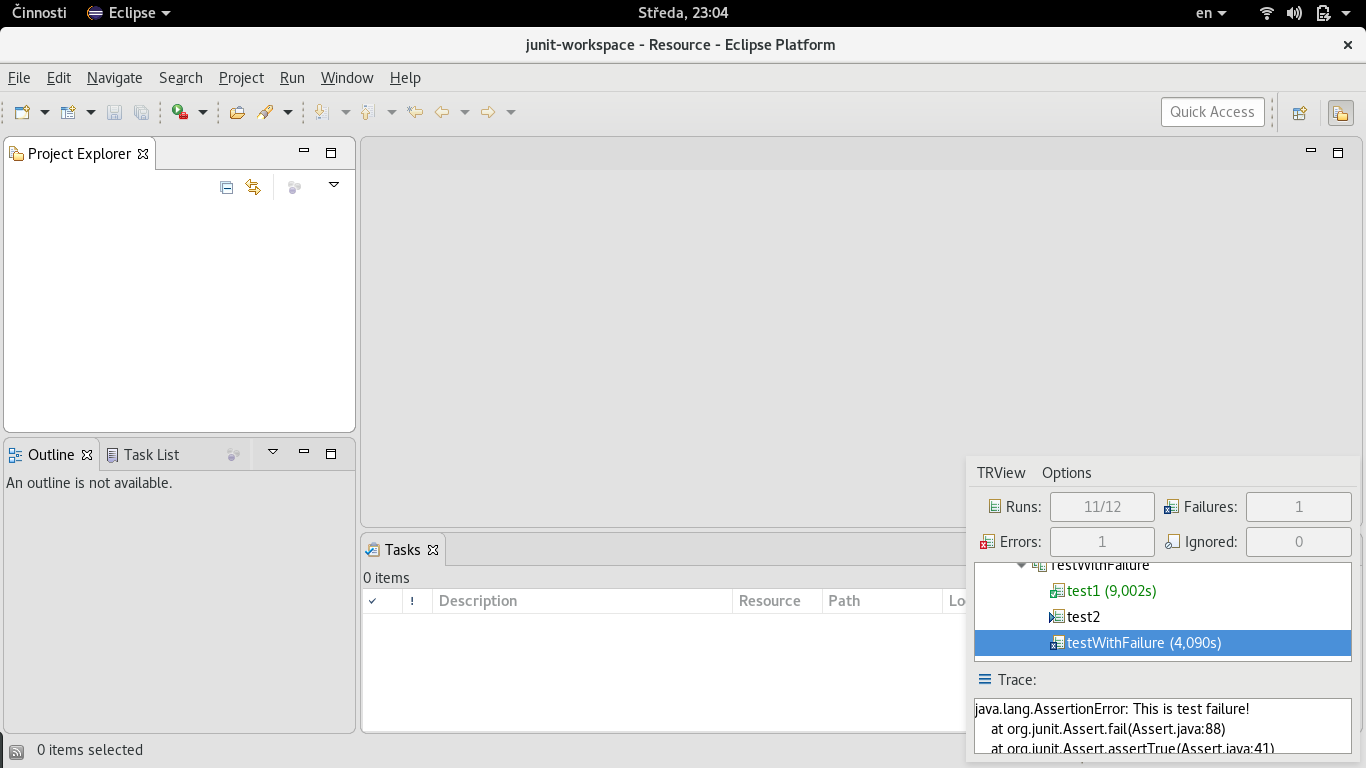
\includegraphics[width=\textwidth, center]{obrazky-figures/TRV_screenshot.png}
    \caption{Snímek obrazovky pořízený při testování GUI Eclipse IDE zobrazující stav běhu testů nástrojem TRV.}
    \label{fig:TRV_screenshot}
  \end{figure}

      \subsection{Instalace aplikace TRV}
      Instalace je odlišná pro obě části nástroje TRV. Zásuvný modul InRunJUnit lze instalovat pomocí Eclipse Update site a aplikaci TRView stačí pouze spustit pomocí JAR archivu.

      \subsubsection{Instalace zásuvného modulu InRunJUnit}
      Pro instalaci zásuvného modulu InRunJUnit je zapotřebí vývojové prostředí Eclipse s JDT. Doporučena je verze Neon (4.6) a vyšší. Instalaci lze provést pomocí \emph{Eclipse Update site} buď z online repositáře, nebo lokálně. Pro instalaci zásuvného modulu InRunJUnit je zatím vytvořen pouze lokální Update site. Z lokálního zdroje lze nainstalovat zásuvný modul pomocí \texttt{Help} -> \texttt{Install New Software...} -> \texttt{Add...} -> \texttt{Local...} , kde se zadá cesta k Eclipse Update site projektu. Ten je dostupný na paměťovém médiu přiloženém k této práci, nebo na webové službě GitHub\footnote{\url{https://github.com/mcoufal/TRV/tree/master/mcoufal.InRunJUnit.updateSite}}.

      \subsubsection{Instalace aplikace TRView}
      Pro spuštění aplikace TRView je zapotřebí pouze stažení JAR archivu a jeho následovné spuštění pomocí javy. Tento archiv je dostupný na paměťovém médiu přiloženém k této práci, nebo webové službě GitHub\footnote{\url{https://github.com/mcoufal/TRV/tree/master/TRView}}. Archiv TRView.jar se nachází ve složce \emph{TRV/TRView} a je možné ho spustit pomocí příkazu '\texttt{java -jar TRView.jar}'.

    \subsection{Použití při testování Eclipse IDE v~Red Hat}
    %******************************************************
    Testování Eclipse IDE probíhá z~velké části automatizovaně. Testovací sady jsou spouštěny oproti jednotlivým verzím operačního systému RHEL a Eclipse IDE. Tyto testy jsou spouštěny buď manuálně, nebo po splnění nastavených podmínek pomocí serveru \emph{Jenkins}\footnote{\url{https://jenkins.io/}}. Testování probíhá na vybraných serverech, které jsou vybrány dle potřeby testera. Testy jsou spuštěny přímo z~konzole\footnote{Příklad spuštění z konzole lze najít na \url{https://wiki.eclipse.org/SWTBot/Automate_test_execution}.} a nevzniká tak druhé okno s~GUI Eclipse IDE. Tento způsob spuštění zachycuje diagram na obrázku \ref{fig:TRV_run_from_term}. Je spuštěna pouze jedna instance Eclipse IDE, se zadanými parametry definujícími mimo jiné umístění pracovní plochy, identifikaci balíčku s implementovanými testy a nastavení parametrů pro cílovou platformu, na které testy poběží. Zásuvný modul InRunJUnit funguje na pozadí v rámci aplikace řídící spuštěné testy.

    \begin{figure}
	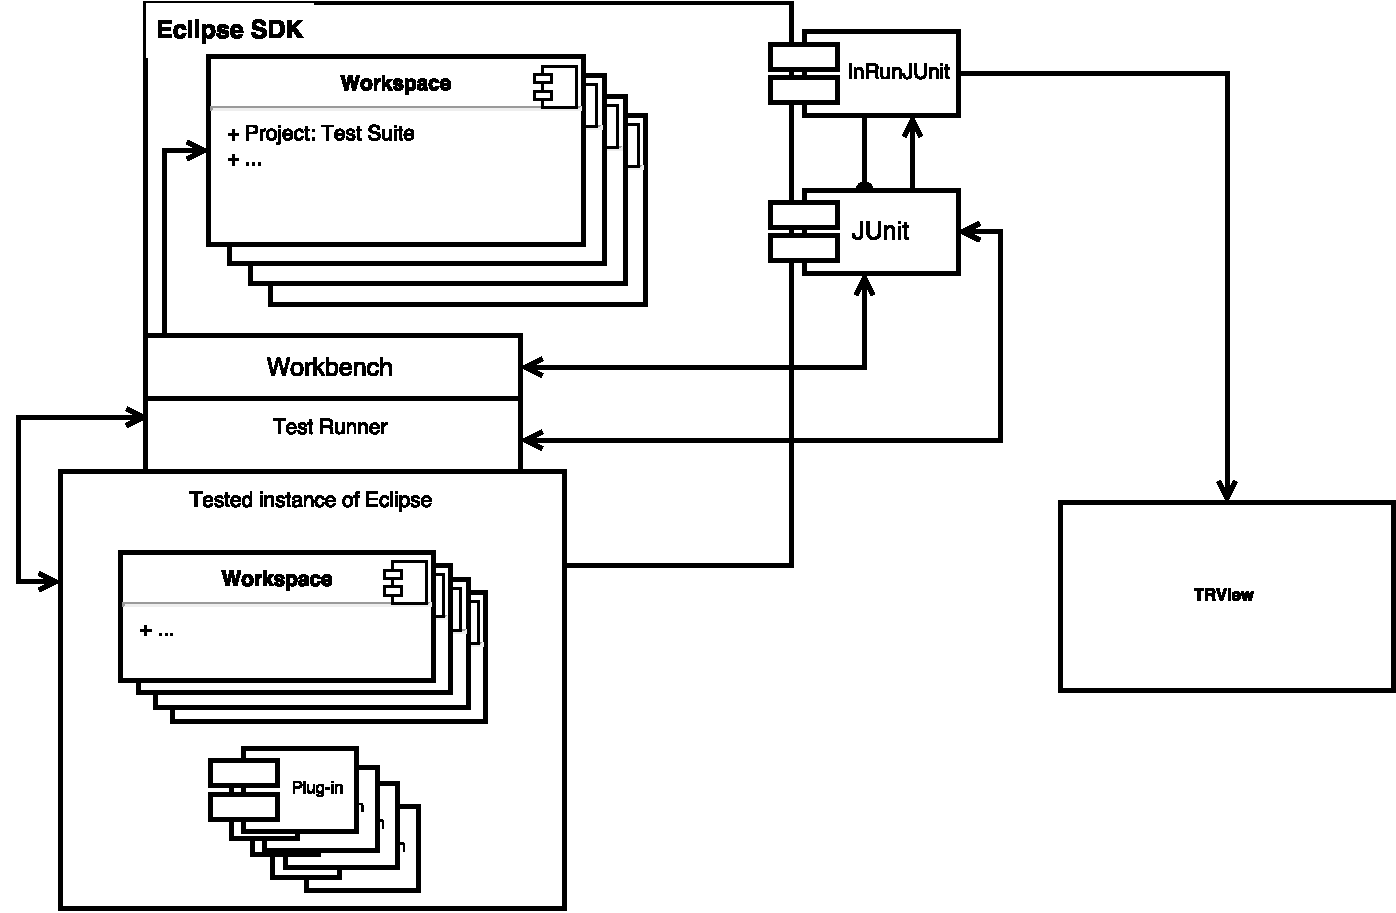
\includegraphics[width=\textwidth, center]{obrazky-figures/TRV_run_from_term.pdf}
	\caption{Znázornění funkce aplikace TRV při spuštění testů z~terminálu.}
	\label{fig:TRV_run_from_term}
      \end{figure}

  \section{Další rozšíření}
  %========================
  Díky obousměrné komunikaci mezi klientskou a serverovou částí má aplikace TRV potenciál na mnohá rozšíření. Užitečnou funkcionalitou by bylo například pozastavení průběhu testů. Uživatel by tak mohl mezitím lépe prozkoumat příčinu neúspěšného testu nebo uvést testovanou instanci do korektního stavu\footnote{Aby nedošlo k~zbytečnému selhání následujících testovacích případů.}. \todo{rozsireni-to co poskytuje JUnit}
  
  \todo{Pokud nejakou funkcionalitu nestihnu - je vhodne ji tady zminit}